\documentclass[12pt,letterpaper, onecolumn]{exam}
\usepackage{amsmath}
\usepackage{amssymb}
\usepackage{sidecap}
\usepackage{tabularx}
\usepackage{csquotes}
\usepackage{makecell}
\usepackage{hyperref}
\hypersetup{
    colorlinks=true,
    linkcolor=blue,
    filecolor=magenta,      
    urlcolor=black,
    pdftitle={Overleaf Example},
    pdfpagemode=FullScreen,
}
%\usepackage[left=0.5cm,right=0.5cm,top=0.5cm,bottom=0.5cm]{geometry}
\usepackage[usestackEOL]{stackengine}
\usepackage{graphicx}
\graphicspath{ {./images/} }
%\setstacktabbedgap{1ex} 
\usepackage{tikz}
\usetikzlibrary{decorations.pathreplacing}
\usetikzlibrary{fadings}
\def\layersep{2.5cm}

\usepackage{enumitem}
\usepackage{algorithm}
\usepackage{algpseudocode}

%\usepackage[shortlabels]{enumitem}
%\usepackage{enumerate}
\usepackage[lmargin=71pt, tmargin=0.8in]{geometry}  %For centering solution box

% \chead{\hline} % Un-comment to draw line below header
\thispagestyle{empty}   %For removing header/footer from page 1

\usepackage{listings}
\usepackage{xcolor}

\definecolor{codegreen}{rgb}{0,0.6,0}
\definecolor{codegray}{rgb}{0.5,0.5,0.5}
\definecolor{codepurple}{rgb}{0.58,0,0.82}
\definecolor{backcolour}{rgb}{0.95,0.95,0.92}

\lstdefinestyle{mystyle}{
    backgroundcolor=\color{backcolour},   
    commentstyle=\color{codegreen},
    keywordstyle=\color{magenta},
    numberstyle=\tiny\color{codegray},
    stringstyle=\color{codepurple},
    basicstyle=\ttfamily\footnotesize,
    breakatwhitespace=false,         
    breaklines=true,                 
    captionpos=b,                    
    keepspaces=true,                 
    numbers=left,                    
    numbersep=5pt,                  
    showspaces=false,                
    showstringspaces=false,
    showtabs=false,                  
    tabsize=2
}

\lstset{style=mystyle}




\begin{document}



\newtheorem{theorem}{Theorem}[section]
\newtheorem{problem}{Problem}
\newtheorem{proposition}{Proposition}[section]
\newtheorem{lemma}{Lemma}[section]
\newtheorem{corollary}[theorem]{Corollary}
\newtheorem{example}{Example}[section]
\newtheorem{definition}[problem]{Definition}

\newcommand{\BEQA}{\begin{eqnarray}}
\newcommand{\EEQA}{\end{eqnarray}}
\newcommand{\define}{\stackrel{\triangle}{=}}
\bibliographystyle{IEEEtran}
\raggedbottom
\setlength{\parindent}{0pt}
\providecommand{\mbf}{\mathbf}
\providecommand{\norm}[1]{\lVert#1\rVert}
\providecommand{\pr}[1]{\ensuremath{\Pr\left(#1\right)}}
\providecommand{\qfunc}[1]{\ensuremath{Q\left(#1\right)}}
\providecommand{\sbrak}[1]{\ensuremath{{}\left[#1\right]}}
\providecommand{\lsbrak}[1]{\ensuremath{{}\left[#1\right.}}
\providecommand{\rsbrak}[1]{\ensuremath{{}\left.#1\right]}}
\providecommand{\brak}[1]{\ensuremath{\left(#1\right)}}
\providecommand{\lbrak}[1]{\ensuremath{\left(#1\right.}}
\providecommand{\rbrak}[1]{\ensuremath{\left.#1\right)}}
\providecommand{\cbrak}[1]{\ensuremath{\left\{#1\right\}}}
\providecommand{\lcbrak}[1]{\ensuremath{\left\{#1\right.}}
\providecommand{\rcbrak}[1]{\ensuremath{\left.#1\right\}}}
\let\vec\mathbf

\newlist{mydesc}{description}{1} % create a new list called mydesc, of type "description"
\setlist[mydesc]{
  align=left, % use the align-format defined above
  leftmargin=0pt, % indentation for all the lines
  labelindent=1em, % horizontal space before label
  labelsep=0pt
   % horizontal space after label -- set to zero because we add space via "leftwithbar"
}



\begingroup  
    \centering
    
    \LARGE Evaluation Metrics\\[0.5em]
    
   % \large Ganji Varshitha\par
   % \large AI20BTECH11009\par
\endgroup
\rule{\textwidth}{0.4pt}
\pointsdroppedatright   %Self-explanatory
\printanswers
\newcommand\Solution{
  \textbf{Solution:}\\}
\newcommand{\myvec}[1]{\ensuremath{\begin{bmatrix}#1\end{bmatrix}}}
 %Replace "Ans:" with starting keyword in solution box

 \subsection*{Metrics}
 \begin{enumerate}
 \item Bias  (Linear Regression) 
\item Coefficient of Determination / R squared (Linear Regression)
\item Adjusted R Squared (Linear Regression)
\item Mean Squared Error (Linear Regression)
\item Root mean Squared Error (Linear Regression)
\item Root Mean Squared Log Error (Linear Regression)
\item Mean Absolute Error (Linear Regression)
\item Explained variance (Linear Regression)
\item Mean Absolute Percentage Error (Linear Regression)
\item AUC ROC (Classification)
\item AUC PR 
\item F measure
\item Accuracy (Classification)
\item Average Precision (Classification)
\item Precision (Classification)
\item Recall (Classification)
\item IoU (Multi-label / Image classification)
\item Confusion Matrix (Classification)
\item ROC curve (Sensitivity/Recall Vs Specificity)
\item PR curve
\item Cumulative gain curve
\item Lift curve
\item Calibration curve
\item Precision by label (Multi-class)
\item Recall by label (Multi-class)
\item F1 score by label (Multi-class)
\item Precision at k (Ranking/ Recommender Systems)
\item Mean Average Precision (Ranking/ Recommender Systems)
\item Normalized Discounted Cumulative Gain (Ranking/ Recommender Systems)
 \end{enumerate}
 
 \newpage
 \subsection*{Bias And Variance}
 
 Statistical or Mathematical models error can be split into reducible and irreducible error. \\Reducible error comprises of 
 \begin{enumerate}
 \item Error due to squared bias
 \item Error due to variance
 \end{enumerate}
 
 \subsubsection*{Bias}
 Bias is the amount that a model’s prediction differs from the target value.\\
 Quantifies how well the model predictions match the ground truths.\\
 If the bias is low, the model matches the training data very well.\\
 However, imagine you could repeat the whole model building process more than once: each time you gather new data and run a new analysis creating a new model.\\ Due to randomness in the underlying data sets, the resulting models will have a range of predictions. Bias measures how far off in general these models' predictions are from the correct value.\\
 Cause: It results from simplifying the assumptions of data used in model so that target function is easier to approximate.\\
 Effects:
 \begin{enumerate}
 \item Underfitting in nature.
 \item Simplified model
 \item High error rate
 \end{enumerate}
 
 \subsubsection*{Variance}
 The error due to variance is taken as the variability of a model prediction for a given data point. Again, imagine you can repeat the entire model building process multiple times. The variance is how much the predictions for a given point vary between different realizations of the model.\\
 High bias will result in low variance which makes the model suboptimal.
 \\
 Causes of high variance: Noisy data set, complex models 
 
 \subsubsection*{Trade-off between Bias and Variance}
 \begin{enumerate}
 \item Increasing complexity of model: Reduces bias and increases variance : Used when model is underfitting.
 \item Increasing the size of dataset: Large dataset tends to generalize easily; Hence, this method is preferred when dealing with overfitting models.
 \item Bagging(\textbf{B}ootstrap \textbf{Agg}regatin\textbf{g}) reduces variance
 \end{enumerate}
 
 \begin{figure}[!h]
 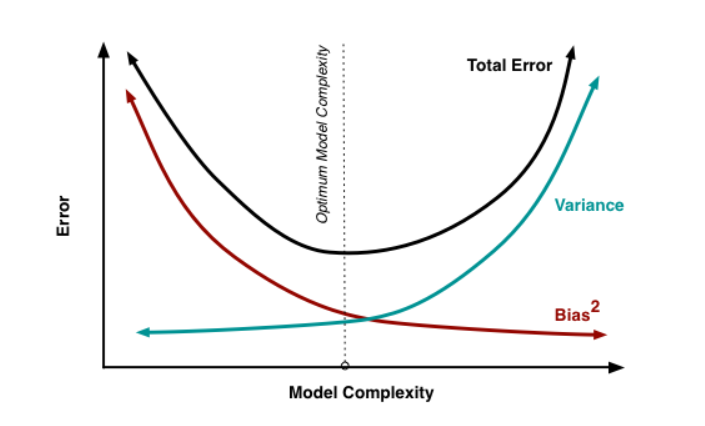
\includegraphics{Bias_Variance_1.png}
 \end{figure}
 
 \subsection*{Coefficient of Determination R-squared Error}
 This metric represents the proportion of variance explained by the model.\\
 R$^{2}$ corresponds to the degree to which the variance in the dependent variable (the target) can be explained by the independent variables (features).
 
 \begin{align*}
 R^2 = {}& 1- \frac{\sum_{i=1}^N(y_i-\hat{y_i})^2}{\sum_{i=1}^N(y_i-\bar{y_i})^2}\\
 ={}& 1 - \frac{(\text{Unexplained Variance})}{(\text{Total Variance})}
 \end{align*}
 
 From the formula, it can be seen comparing the fit of the model with simple mean model where the prediction for each observation is same as the mean of all observations.\\
 Dependent variable(y) has variance $\frac{\sum_{i=1}^N(y_i-\bar{y_i})^2}{N}$ which cannot be explained by the simple model.\\
 Higher R$^{2}$ value means a greater fit.\\
 It assumes every feature helps in explaining the variation in target.\\ If not linear model,  R$^{2}$ may be negative.  
 \\ 
 It does not determine the goodness of fit of the model.
 Since it does not give any measure of bias, highly overfitted model may have higher R$^{2}$.
 
 \subsection*{Adjusted R squared}
 Since R$^{2}$ metric assumes every feature helps in explaining the variance, it might explain 100$\%$ of variance but in reality it is not learning but overfitting.\\
 Hence, we penalise adding features that are not useful for predicting the target. The value of the adjusted  R$^{2}$ decreases if the increase in the  R$^{2}$ caused by adding new features is not significant enough.
 \begin{align*}
 R_a^2 ={}&  1-[\frac{(n-1)}{(n-k-1)}(1-R^2)]
 \end{align*}
 where n  is number of observations and k is number of independent variables.
 
 
 







\end{document}